% Source: https://scnajei2ds6y.feishu.cn/wiki/SXzcw2VtHig3bPkRfIickYa8nVh
% Faithful reproduction; figures captured from the rendered Feishu page after original-media download timed out.
\documentclass[zihao=false,fontset=windows]{ctexart}
% ctexart 不接受任意 pt 选项。正文改 {10pt}，方括号里是行距。
\usepackage{scrextend}
\changefontsizes[12pt]{10pt}

\usepackage[a4paper,left=2.35cm,right=2.35cm,top=1.7cm,bottom=1.9cm]{geometry}
\usepackage{xcolor}
\usepackage{graphicx}
\usepackage{amsmath,amssymb}
\usepackage{enumitem}
\usepackage{needspace}
\usepackage{tabularx}
\usepackage{colortbl}
\usepackage{listings}
\usepackage{hyperref}
\usepackage[most]{tcolorbox}

\definecolor{feishuText}{RGB}{31,35,41}
\definecolor{feishuBlue}{RGB}{36,91,219}
\definecolor{feishuRed}{RGB}{216,57,49}
\definecolor{feishuGray}{RGB}{100,106,115}
\definecolor{feishuGray2}{RGB}{143,149,158}
\definecolor{feishuPinkBg}{RGB}{251,191,188}
\definecolor{quoteBar}{RGB}{51,112,255}
\definecolor{codebg}{RGB}{245,246,247}
\definecolor{codeborder}{RGB}{222,224,227}
\definecolor{inlinebg}{RGB}{242,243,245}
\definecolor{callRed}{RGB}{253,226,226}
\definecolor{callOrange}{RGB}{255,245,235}
\definecolor{callYellow}{RGB}{254,255,240}
\definecolor{callGreen}{RGB}{240,251,239}
\definecolor{callBlue}{RGB}{240,244,255}
\definecolor{callRedSoft}{RGB}{254,241,241}
\definecolor{callSun}{RGB}{255,255,204}
\definecolor{tableHead}{RGB}{242,243,245}
\definecolor{tableRule}{RGB}{222,224,227}
\definecolor{codeText}{RGB}{31,35,41}
\definecolor{codeKeyword}{RGB}{0,0,255}
\definecolor{codeComment}{RGB}{0,128,0}
\definecolor{codeString}{RGB}{163,21,21}

\setmainfont{Times New Roman}
\setCJKmainfont{Microsoft YaHei}[AutoFakeBold=2.2]
\setCJKsansfont{Microsoft YaHei}[AutoFakeBold=2.2]
\setCJKmonofont{Microsoft YaHei}[AutoFakeBold=2.2]
\setmonofont{Consolas}
\newfontfamily\emojifont{Segoe UI Emoji}

\hypersetup{
  colorlinks=true,
  urlcolor=feishuBlue,
  linkcolor=feishuBlue,
  unicode=true,
  pdftitle={InternViT}
}

\setlength{\parindent}{0pt}
\setlength{\parskip}{0.42em}
\setlength{\fboxsep}{1.5pt}
\setlength{\emergencystretch}{3em}
\linespread{1.28}
\color{feishuText}
\arrayrulecolor{tableRule}
\urlstyle{same}

\setlist[enumerate]{label=\textcolor{feishuBlue}{\arabic*.}, leftmargin=1.7em, itemsep=0.22em, topsep=0.28em, parsep=0.08em, partopsep=0pt}
\setlist[itemize,1]{label=\textcolor{feishuBlue}{\textbullet}, leftmargin=1.35em, itemsep=0.18em, topsep=0.25em, parsep=0.06em, partopsep=0pt}
\setlist[itemize,2]{label=\textcolor{feishuBlue}{◦}, leftmargin=1.45em, itemsep=0.12em, topsep=0.15em}
\setlist[itemize,3]{label=\textcolor{feishuBlue}{\rule[0.18em]{0.38em}{0.38em}}, leftmargin=1.55em, itemsep=0.1em, topsep=0.12em}

\newcommand{\feiEmoji}[1]{{\emojifont #1}}
\newcommand{\incode}[1]{\colorbox{inlinebg}{\ttfamily\small #1}}
\newcommand{\bigmath}[1]{%
  \begin{center}\large$\displaystyle #1$\end{center}%
}

\lstset{
  language=Python,
  basicstyle=\ttfamily\footnotesize\color{codeText},
  keywordstyle=\color{codeKeyword},
  commentstyle=\color{codeComment},
  stringstyle=\color{codeString},
  showstringspaces=false,
  breaklines=true,
  columns=fullflexible,
  keepspaces=true,
  tabsize=4,
  upquote=true,
  aboveskip=2pt,
  belowskip=0pt,
  xleftmargin=0pt,
  frame=none
}

\tcbset{
  feishubase/.style 2 args={
    enhanced,
    boxrule=0pt,
    arc=8pt,
    left=10pt,
    right=10pt,
    top=7pt,
    bottom=7pt,
    before skip=6pt,
    after skip=6pt,
    colback=#1,
    colframe=#1,
    before upper={\feiEmoji{#2}\hspace{0.45em}\ignorespaces}
  }
}
\newtcolorbox{feishubox}[2]{feishubase={#1}{#2}, breakable}
\newtcolorbox{feishuboxnb}[2]{feishubase={#1}{#2}}

\newtcolorbox{feishuquote}{
  enhanced,
  breakable,
  boxrule=0pt,
  leftrule=3pt,
  arc=0pt,
  colframe=quoteBar,
  colback=white,
  left=8pt,
  right=2pt,
  top=2pt,
  bottom=2pt,
  before skip=4pt,
  after skip=4pt,
  before upper=\color{feishuGray}
}

\newtcolorbox{feishucode}{
  enhanced,
  breakable,
  colback=codebg,
  colframe=codeborder,
  boxrule=0.6pt,
  arc=6pt,
  left=6pt,
  right=6pt,
  top=5pt,
  bottom=4pt,
  before skip=6pt,
  after skip=6pt
}

\begin{document}
{\zihao{1}\bfseries InternViT\par}
% source block 2
\begin{feishubox}{callOrange}{☘}
论文：\href{https://arxiv.org/pdf/2312.14238}{《InternVL: Scaling up Vision Foundation Models and Aligning for Generic Visual-Linguistic Tasks》}\par
模型仓库：\href{https://huggingface.co/collections/OpenGVLab/internvl10-65b92d6be81c86166ca0dde4}{OpenGVLab}\href{https://huggingface.co/collections/OpenGVLab/internvl10-65b92d6be81c86166ca0dde4}{/InternVL1.0}\par
\end{feishubox}

% source block 5
InternViT 是 InternVL 系列多模态大模型（\href{https://scnajei2ds6y.feishu.cn/wiki/IOYWwSHmKib7TokydUdcHxFznIU}{InternVL 3}、\href{https://scnajei2ds6y.feishu.cn/wiki/JDc4wjjcIiKRhtkXj45cT78fnz9}{InternVL 3.5}）的视觉编码器。\par
% source block 6
在模型结构上，InternViT 相比早期的 \href{https://scnajei2ds6y.feishu.cn/wiki/QEJ8wXq9GiTBrxkMqbScnd8nnod}{ViT(2020, Google Research)}结构，融合了 RMSNorm、QK Norm、LayerScale、DropPath、FlashAttention 等多项现代 Transformer 架构技术。\par
% source block 7
在模型训练上，InternViT \textcolor{feishuRed}{融合了对比学习任务和生成任务}，生成任务参考了\href{https://scnajei2ds6y.feishu.cn/wiki/AZiVwFmXEirI77kAVzYcOMNVnbh}{BLIP-2(2023, Salesforce Research)}的Qformer训练模式（参考\href{https://scnajei2ds6y.feishu.cn/wiki/Lu0owe0xii7LjmkfyNzc0mdjnEh}{MLP vs. Q-Former}），但是又可以灵活遵循\href{https://scnajei2ds6y.feishu.cn/wiki/HTJVw44IJibX6gkYWtlc1zCYnVh}{LLaVA-1.5(2023, Microsoft Research)}方案对齐。\par
% source block 8
\par\vspace{0.95em}\noindent{\zihao{-2}\bfseries \textcolor{feishuBlue}{1.} 模型架构}\par\vspace{0.28em}
% source block 9
整体是一个 ViT 编码器结构（Vision Transformer Encoder），包括：\par
% source block 10
\begin{itemize}
\item Patch Embedding
\end{itemize}
% source block 11
\begin{itemize}
\item Transformer Encoder
\end{itemize}
% source block 12
\begin{itemize}
\item 输出整合（[cls]、last\_hidden\_state）
\end{itemize}
% source block 13
但 InternViT 相比早期的 \href{https://scnajei2ds6y.feishu.cn/wiki/QEJ8wXq9GiTBrxkMqbScnd8nnod}{ViT(2020, Google Research)}结构，融合了 RMSNorm、QK Norm、LayerScale、DropPath、FlashAttention 等多项现代 Transformer 架构技术。\par
% source block 14

% source block 15
\par\vspace{0.95em}\noindent{\zihao{3}\bfseries \textcolor{feishuBlue}{1.1} RMSNorm}\par\vspace{0.28em}
% source block 16
\textbf{\textcolor{feishuRed}{LLaMA以来的大模型大多都使用RMSNorm。}}\textbf{\textcolor{feishuRed}{\href{https://scnajei2ds6y.feishu.cn/wiki/BHRrwQ4TAi9iCskVsMccByePngc}{Qwen2-VL}}}\textbf{\textcolor{feishuRed}{也在ViT上使用RMSNorm让ViT更接近语言模型架构。}}\par
% source block 17
RMSNorm通过均方根值缩放输入，保留原始均值信息，其公式是：\par
% source block 18
\bigmath{y_i=\frac{x_i}{\operatorname{RMS}(x)}*\gamma_i,\ \text{where }\operatorname{RMS}(x)=\sqrt{\epsilon+\frac{1}{n}\sum_{i=1}^{n}x_i^2}}
% source block 19
其中RMS是在最后一个维度(hidden\_dim)上进行计算的。可训练参数为向量$\gamma$。\par
% source block 20
\begin{feishucode}
\lstset{moredelim=[is][\bfseries\color{feishuRed}]{@!}{!@}}
\begin{lstlisting}[numbers=left,numberstyle=\tiny\color{feishuGray},numbersep=6pt,xleftmargin=12pt]
class InternRMSNorm(nn.Module):
    def __init__(self, hidden_size, eps=1e-6):
        super().__init__()
        self.weight = nn.Parameter(torch.ones(hidden_size))
        self.variance_epsilon = eps

    def forward(self, hidden_states):
        input_dtype = hidden_states.dtype
        hidden_states = hidden_states.to(torch.float32)
        variance = hidden_states.pow(2).mean(-1, keepdim=True)
        hidden_states = hidden_states * torch.rsqrt(variance + self.variance_epsilon)
        return self.weight * hidden_states.to(input_dtype)
\end{lstlisting}
\end{feishucode}

% source block 21

% source block 22
\par\vspace{0.95em}\noindent{\zihao{3}\bfseries \textcolor{feishuBlue}{1.2} QK Norm}\par\vspace{0.28em}
% source block 23
QK Norm是近期开源的文本大模型使用的技术，目标是为了\textcolor{feishuRed}{降低数值波动、提升稳定性（使 Softmax 函数在不牺牲表达能力的情况下不那么容易出现饱和）。}\par
% source block 24
做法上是在Q、K上分别做 L2 Norm 实现把 Q、K 两个 vector（这里是逐token计算视角，因此是vector）转化为单位向量，这样的话QK的单点乘积就可以变成$Q'K'^{T}=\mathit{cosine\_similarity}(Q',K')$\par
% source block 25
其中 $Q'=Q/\lVert Q\rVert$，$K'=K/\lVert K\rVert$，\textcolor{feishuRed}{而}$\mathit{cosine\_similarity}$\textcolor{feishuRed}{是限制在}$[-1,1]$\textcolor{feishuRed}{的，避免出现Softmax饱和问题。}\par
% source block 26
\begin{feishucode}
\lstset{moredelim=[is][\bfseries\color{feishuRed}]{@!}{!@}}
\begin{lstlisting}[numbers=left,numberstyle=\tiny\color{feishuGray},numbersep=6pt,xleftmargin=12pt]
class InternAttention(nn.Module):
    """Multi-headed attention from 'Attention Is All You Need' paper"""

    def __init__(self, config: InternVisionConfig):
        self.qkv = nn.Linear(self.embed_dim, 3 * self.embed_dim, bias=config.qkv_bias)
        self.attn_drop = nn.Dropout(config.attention_dropout)
        self.proj_drop = nn.Dropout(config.dropout)

        self.qk_normalization = config.qk_normalization

@!        if self.qk_normalization:!@
@!            self.q_norm = InternRMSNorm(self.embed_dim, eps=config.layer_norm_eps)!@
@!            self.k_norm = InternRMSNorm(self.embed_dim, eps=config.layer_norm_eps)!@

    def _naive_attn(self, x):
        B, N, C = x.shape
        qkv = self.qkv(x).reshape(B, N, 3, self.num_heads, C // self.num_heads).permute(2, 0, 3, 1, 4)
        q, k, v = qkv.unbind(0)  # make torchscript happy (cannot use tensor as tuple)

        if self.qk_normalization:
            B_, H_, N_, D_ = q.shape
@!            q = self.q_norm(q.transpose(1, 2).flatten(-2, -1)).view(B_, N_, H_, D_).transpose(1, 2)!@
@!            k = self.k_norm(k.transpose(1, 2).flatten(-2, -1)).view(B_, N_, H_, D_).transpose(1, 2)!@

        attn = ((q * self.scale) @ k.transpose(-2, -1))
\end{lstlisting}
\end{feishucode}

% source block 27

% source block 28
\par\vspace{0.95em}\noindent{\zihao{3}\bfseries \textcolor{feishuBlue}{1.3} LayerScale \& DropPath}\par\vspace{0.28em}
% source block 29
DropPath 和 Dropout 一样也是正则化方法。\par
% source block 30
传统的 Dropout 是在 \textbf{神经元层面} 随机丢弃激活值，而 DropPath 是在 \textbf{\textcolor{feishuRed}{网络路径（整层残差分支）层面}} 随机丢弃。也就是说，在每次前向传播中：\par
% source block 31
\begin{itemize}
\item 某些残差连接（Residual Branch）会被随机关闭；
\end{itemize}
% source block 32
\begin{itemize}
\item 相当于\textcolor{feishuRed}{“跳过”}某一层的 Transformer block；
\end{itemize}
% source block 33
\begin{itemize}
\item 从而让不同样本看到的模型结构略有不同。
\end{itemize}
% source block 34
而且在DropPath中，InternViT还使用了两组可学习LayerScale：\incode{self.ls1}和 \incode{self.ls2}：\par
% source block 35
\begin{feishucode}
\lstset{moredelim=[is][\bfseries\color{feishuRed}]{@!}{!@}}
\begin{lstlisting}[numbers=left,numberstyle=\tiny\color{feishuGray},numbersep=6pt,xleftmargin=12pt]
class InternVisionEncoderLayer(nn.Module):
    def __init__(self, config: InternVisionConfig, drop_path_rate: float):
        super().__init__()
        self.embed_dim = config.hidden_size
        self.intermediate_size = config.intermediate_size

        self.attn = InternAttention(config)
        self.mlp = InternMLP(config)
        self.norm1 = InternRMSNorm(self.embed_dim, eps=config.layer_norm_eps)
        self.norm2 = InternRMSNorm(self.embed_dim, eps=config.layer_norm_eps)

        self.ls1 = nn.Parameter(config.initializer_factor * torch.ones(self.embed_dim))
        self.ls2 = nn.Parameter(config.initializer_factor * torch.ones(self.embed_dim))
        self.drop_path1 = DropPath(drop_path_rate) if drop_path_rate > 0. else nn.Identity()
        self.drop_path2 = DropPath(drop_path_rate) if drop_path_rate > 0. else nn.Identity()

    def forward(
            self,
            hidden_states: torch.Tensor,
    ) -> Tuple[torch.FloatTensor, Optional[torch.FloatTensor], Optional[Tuple[torch.FloatTensor]]]:
        """
        Args:
            hidden_states (`Tuple[torch.FloatTensor, Optional[torch.FloatTensor]]`): input to the layer of shape `(batch, seq_len, embed_dim)`
        """
@!        hidden_states = hidden_states + self.drop_path1(self.attn(self.norm1(hidden_states)) * self.ls1)!@

@!        hidden_states = hidden_states + self.drop_path2(self.mlp(self.norm2(hidden_states)) * self.ls2)!@

        return hidden_states
\end{lstlisting}
\end{feishucode}

% source block 68

% source block 36

% source block 37
值得注意的是，InternViT使用的位置编码和 \href{https://scnajei2ds6y.feishu.cn/wiki/QEJ8wXq9GiTBrxkMqbScnd8nnod}{ViT(2020, Google Research)}一样仍然是 \textbf{\textcolor{feishuRed}{可学习的（learnable）绝对位置编码}}\textbf{，}参考\href{https://scnajei2ds6y.feishu.cn/wiki/O2arwxGNXi6KrckUG1dcGcbrnWd}{ViT的位置编码}\textbf{：}\par
% source block 38
\begin{feishucode}
\lstset{moredelim=[is][\bfseries\color{feishuRed}]{@!}{!@}}
\begin{lstlisting}[numbers=left,numberstyle=\tiny\color{feishuGray},numbersep=6pt,xleftmargin=12pt]
self.position_embedding = nn.Parameter(
    torch.randn(1, self.num_positions, self.embed_dim)
)
\end{lstlisting}
\end{feishucode}

% source block 39

% source block 40
\par\vspace{0.95em}\noindent{\zihao{-2}\bfseries \textcolor{feishuBlue}{2.} 训练}\par\vspace{0.28em}
% source block 41
InternViT的训练通过QLLaMA中间件对齐视觉与语言特征空间，从\textcolor{feishuRed}{对比学习到生成学习}的策略演进，有效利用不同质量数据。三个阶段分别采用\textcolor{feishuRed}{196/224/364}像素分辨率。\par
% source block 42
\begin{center}
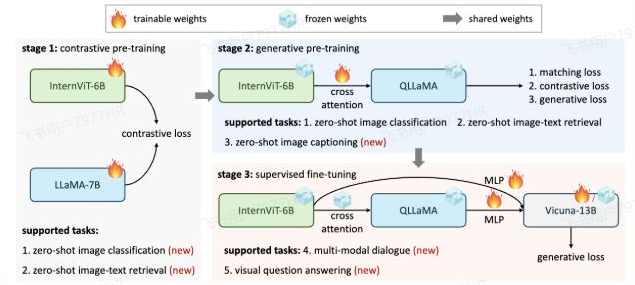
\includegraphics[width=0.98\textwidth]{images/InternViT/fig-01.png}
\end{center}
% source block 43
\par\vspace{0.95em}\noindent{\zihao{3}\bfseries \textbf{Stage 1：视觉-语言对比训练}}\par\vspace{0.28em}
% source block 44
\begin{enumerate}[start=1]
\item \textbf{模型初始化}：图像编码器InternViT-6B采用BEiT初始化方法随机初始化，文本编码器LLaMA-7B加载多语言预训练权重，\textcolor{feishuRed}{全部参数可训练}。
\end{enumerate}
% source block 45
\begin{enumerate}[start=2]
\item \textbf{数据与优化}：使用 4.98B 过滤后的图像-文本对（来源包括LAION-en, LAION-multi, LAION-COCO, COYO, Wukong等），采用AdamW优化器（$\beta$1=0.9, $\beta$2=0.95），图像/文本编码器初始学习率分别为1e-3/1e-4，cosine衰减LR。
\end{enumerate}
% source block 46
\begin{enumerate}[start=3]
\item 初始化196$\times$196分辨率训练时掩码50\%图像token。最后0.5B训练数据过渡到224$\times$224分辨率阶段，取消掩码。
\end{enumerate}
% source block 47

% source block 48
\par\vspace{0.95em}\noindent{\zihao{3}\bfseries \textbf{Stage 2：视觉-语言生成训练}}\par\vspace{0.28em}
% source block 49
这里引入了一个QLLaMA权重，这是一个经过视觉语言对齐的LLaMA权重。\par
% source block 50
\begin{enumerate}[start=1]
\item \textbf{参数冻结}：InternViT-6B和QLLaMA冻结权重，仅训练新增的96个可学习查询和交叉注意力层（本质就是Q-Former结构，1B参数）。
\end{enumerate}
% source block 51
\begin{enumerate}[start=2]
\item \textbf{数据升级}：使用严格过滤后的1.03B 高质量图文对，包含ITC/ITM/ITG综合损失，参考\href{https://scnajei2ds6y.feishu.cn/wiki/AZiVwFmXEirI77kAVzYcOMNVnbh}{BLIP-2(2023, Salesforce Research)}。
\end{enumerate}
% source block 52
\begin{enumerate}[start=3]
\item AdamW优化器（$\beta$1=0.9, $\beta$2=0.98），峰值学习率5e-5，20K batchsize。
\end{enumerate}
% source block 53

% source block 54
\par\vspace{0.95em}\noindent{\zihao{3}\bfseries \textbf{Stage 3：监督微调}}\par\vspace{0.28em}
% source block 55
\begin{enumerate}[start=1]
\item \textbf{两种配置}：
\begin{itemize}
\item (a) 独立使用InternViT-6B：遵循\href{https://scnajei2ds6y.feishu.cn/wiki/HTJVw44IJibX6gkYWtlc1zCYnVh}{LLaVA-1.5(2023, Microsoft Research)}方案，分两阶段微调MLP层和LLM。
\item (b) 全模型整合：结合InternViT-6B和QLLaMA（本身可以看作一个大型Q-Former），扩展数据集至4M样本，批量增至512。
\end{itemize}
\end{enumerate}
% source block 56
\begin{enumerate}[start=2]
\item \textbf{训练策略}：
\begin{itemize}
\item 使用混合\textbf{\textcolor{feishuRed}{指令}}数据集（COCO Caption、VQAv2等）
\item （可选）冻结LLM解码器训练，保留原始语言能力。
\end{itemize}
\end{enumerate}
% source block 57
这里读者可能有点疑惑这个InternViT-6B+QLLaMA如何使用，这个看下面这个使用场景图就知道，(c)就是直接使用InternViT-6B、(d)是使用InternViT-6B+QLLaMA：\par
% source block 58
\begin{center}
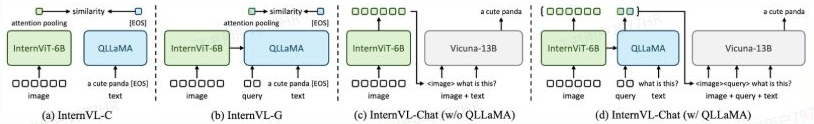
\includegraphics[width=0.98\textwidth]{images/InternViT/fig-02.png}
\end{center}
% source block 59

% source block 60
\Needspace{8cm}
\par\vspace{0.95em}\noindent{\zihao{-2}\bfseries \textcolor{feishuBlue}{3.} 实验}\par\vspace{0.28em}
% source block 61
论文里关注了classification、image-text retrieval这样的ViT传统benchmark，我们主要关注多模态理解生成的表现：\par
% source block 62
\begin{center}
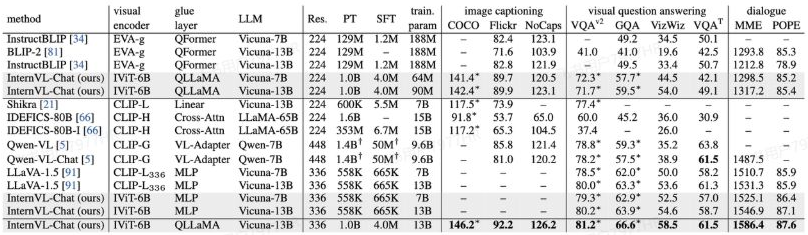
\includegraphics[width=0.98\textwidth]{images/InternViT/fig-03.png}
\end{center}
% source block 63

\end{document}